\hypertarget{a00007}{
\section{Dokumentacja pliku /home/pawel/Dokumenty/Uczelnia/grupappz/Source/Ass8-server/parser.cpp}
\label{a00007}\index{/home/pawel/Dokumenty/Uczelnia/grupappz/Source/Ass8-server/parser.cpp@{/home/pawel/Dokumenty/Uczelnia/grupappz/Source/Ass8-server/parser.cpp}}
}
{\tt \#include $<$iostream$>$}\par
{\tt \#include $<$string$>$}\par
{\tt \#include $<$cstdlib$>$}\par
{\tt \#include $<$cstdio$>$}\par
{\tt \#include $<$vector$>$}\par
{\tt \#include $<$sys/types.h$>$}\par
{\tt \#include $<$unistd.h$>$}\par
{\tt \#include $<$sys/wait.h$>$}\par
{\tt \#include \char`\"{}version.h\char`\"{}}\par
{\tt \#include \char`\"{}parser.hpp\char`\"{}}\par
{\tt \#include \char`\"{}xml.hpp\char`\"{}}\par
{\tt \#include \char`\"{}debug.hpp\char`\"{}}\par


Wykres zależności załączania dla parser.cpp:\nopagebreak
\begin{figure}[H]
\begin{center}
\leavevmode
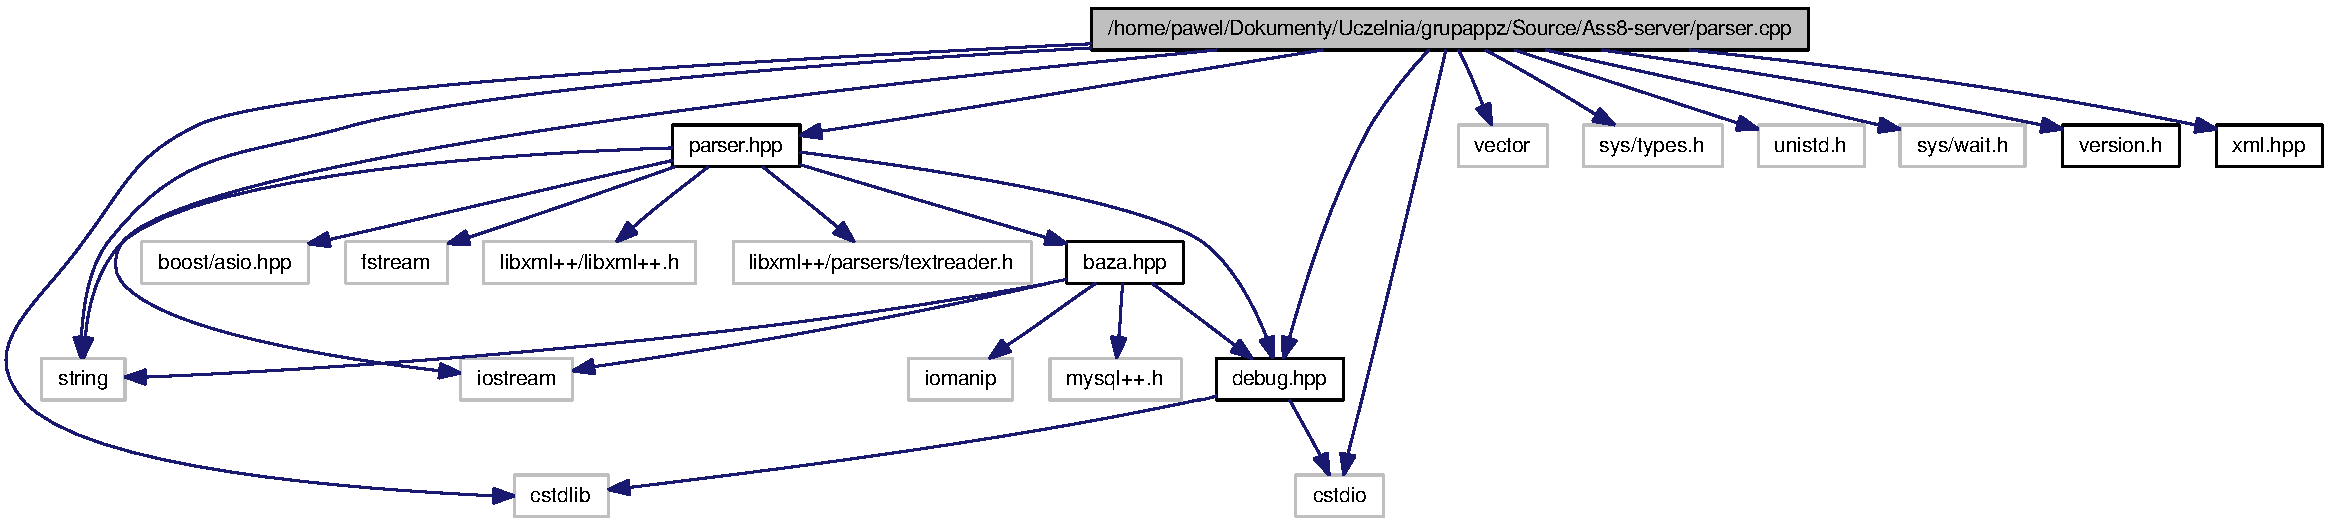
\includegraphics[width=420pt]{a00029}
\end{center}
\end{figure}
